\subsection{Existence of adversarial examples}
\subsubsection{ Description of the experience}

\href{https://github.com/LIUHanlin16895/MLA_projet/blob/main/src/existence_adv/GoogLeNet_existence_adv_examples.ipynb}{Lien github: GoogLeNet}

\textit{Explaining and Harnessing Adversarial Examples}\citep{goodfellow2014explaining}, a classic paper in the field of adversarial examples, the most widely known of which is Szegedy et al.'s proof of the existence of adversarial examples and the validity of FGSM on GooLeNet.

\FloatBarrier
\begin{figure}[htbp]%插入图片
        \centering
        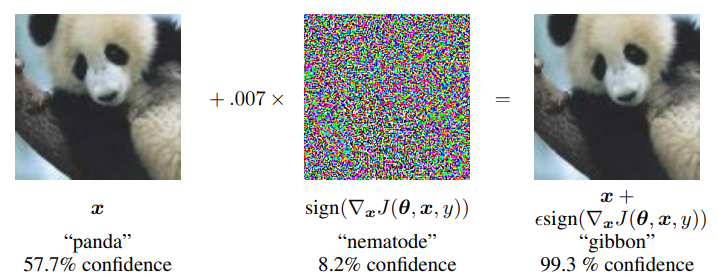
\includegraphics[scale=0.3]{imagePanda.png}%height=2cm,width=3cm,
        \caption{ A demonstration of fast adversarial example generation applied to GoogLeNet (Szegedy et al., 2014a) on ImageNet.}
        \label{panda}
\end{figure}\par
\FloatBarrier

By adding an imperceptibly small vector whose elements are equal to the sign of the elements of the gradient of the cost function with respect to the input, we can change GoogLeNet’s classification of the image. (cf.FIGURE \ref{panda}) 

GoogLeNet is one of the most successful models of the earlier years of convolutional neural networks and is a type of convolutional neural network based on the Inception architecture. It utilises Inception modules, which allow the network to choose between multiple convolutional filter sizes in each block. As mentioned above, we do not currently have a license for ImagNet, so the entire test will be conducted on the Mnist dataset. After building and training the GooLeNet network, we obtained an accuracy of 98\% on the valid set. (cf.FIGURE \ref{GLN})

\FloatBarrier
\begin{figure}[htbp]%插入图片
        \centering
        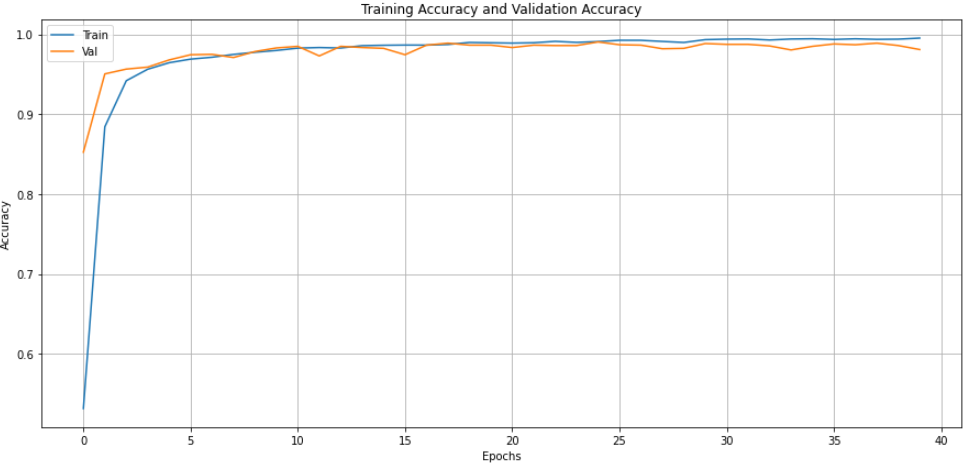
\includegraphics[scale=0.25]{GLNtrainingAcc.PNG}%height=2cm,width=3cm,
        \caption{ Accuracy of GoogLeNet on the training set and valid set}
        \label{GLN}
\end{figure}\par
\FloatBarrier

We will then do two tests, firstly, to confirm that the adversarial examples do have an effect on the network, and to observe the confidence level of the network classification results. Secondly, observe the effect of different levels of interference on the accuracy of the network.
\subsubsection{Results}
After generating the model, we first generated a sample adversarial case using the FGSM method (cf.FIGURE\ref{adv_exp}). We note that this adversarial examples is of the same form as the image in the article but of a different size, due to the size of the image in the database.
\FloatBarrier
\begin{figure}[htbp]
        \centering
        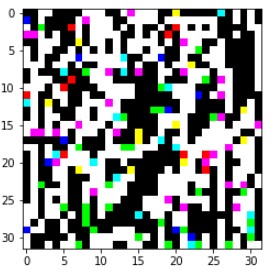
\includegraphics[scale=0.25]{adv_exp.PNG}%height=2cm,width=3cm,
        \caption{Adversarial examples generated by GoogLeNet on Mnist}
        \label{adv_exp}
\end{figure}\par
\FloatBarrier

In \cite{szegedy2013intriguing}, a mere 0.007 ($\epsilon=0.007$) interference on the imageNet dataset was used to give the network 99.3\% confidence that its incorrect judgments were correct (cf.FIGURE\ref{panda}). Due to the different datasets used, the interference reached 0.2 ($\epsilon=0.2$)before the network was nearly 100\% confident that an incorrect decision was made. However, this still confirms that an adversarial examples of only 0.2 per cent can make the network completely wrong. (cf.FIGURE \ref{GLN_without_adv} and \ref{GLN_with_adv})

\begin{figure}[htbp]
\centering
\begin{minipage}[t]{0.48\textwidth}
\centering
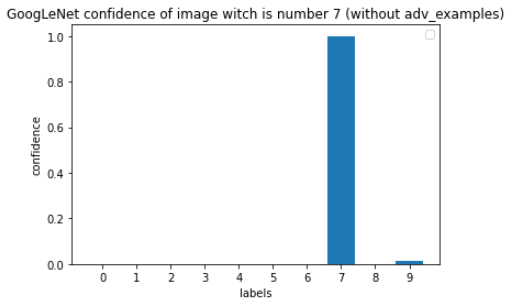
\includegraphics[width=6 cm]{GLN confiance without adv 7.png}
\caption{GoogLeNet confidence without adv examples}
\label{GLN_without_adv}
\end{minipage}
\begin{minipage}[t]{0.48\textwidth}
\centering
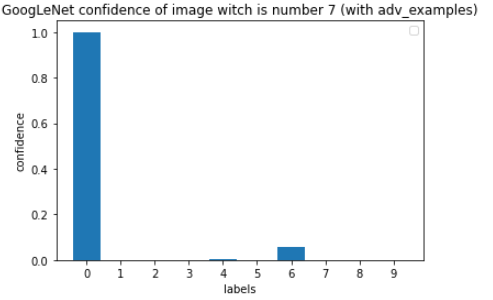
\includegraphics[width=6cm]{GLN confiance with adv 7.png}
\caption{GoogLeNet confidence with adv examples}
\label{GLN_with_adv}
\end{minipage}
\end{figure}
Next we observed the effect of different magnitudes of interference on the accuracy of the network, accuracy does decrease with increasing interference. (cf.FIGURE \ref{acc_GLN}) Only 0. 1 perturbation is needed to reduce the accuracy of the network to 45\%.
\FloatBarrier
\begin{figure}[htbp]
        \centering
        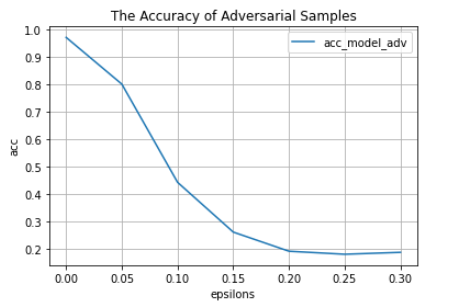
\includegraphics[width=6cm]{Acc of GLN with adv exp.PNG}%height=2cm,width=3cm,
        \caption{Accurcy of GoogLeNet with increasing interference}
        \label{acc_GLN}
\end{figure}\par
\FloatBarrier

\subsubsection{Discussion}
Through the above experiments, we learned about the existence of adversarial examples and succeeded in verifying the explanation in the paper: the accuracy of the input features of a neural network is finite, and if a perturbation is smaller than that accuracy, the classifier ignores the perturbation. But the change in activation caused by perturbation can grow linearly with dimensionality. For higher dimensional problems, if there are small changes to the input, then these add up to a large change to the output.

For a high performance network like GoogLeNet a perturbation of only 0.2 is needed to give 100\% confidence in a wrong decision, while a perturbation of 0.3 gives an accuracy of only 0.2.

\subsection{Linear Model}
\subsubsection{Description of the experience}
\href{https://github.com/LIUHanlin16895/MLA_projet/blob/main/src/softmax/ProjetMLA_Softmax.ipynb}{Lien github: Softmax}

\href{https://github.com/LIUHanlin16895/MLA_projet/blob/main/src/logistic_regression/ProjetMLA_LogisticRegression.ipynb}{Lien github: Logistic regression} \\

After discussing the existence of adversarial examples and how the FGSM algorithm can quickly generate adversarial-like examples, the article first applies the FGSM method on the simplest logistic regression model so as to understand how to generate adversarial examples in a simple setting. 

It is supposed in the article that we train a single model to recognize labels $y\in${-1,1} with $P(y=1) = \sigma(\omega^Tx+b)$ where $\sigma(z)$ is the logistic sigmoid function, then training consists of gradient descent on $$\mathbb{E}_{x,y\sim p_{data}}\zeta(-y(\omega^Tx+b))$$ where $\zeta(z)=log(1+exp(z))$ is the softplus function. 

We can derive a simple analytical form for training on \textbf{the worst-case} adversarial perturbation of $x$ rather than $x$ itself, based on gradient sign perturbation. Using the FGSM method for this model, the perturbations $$\eta = \epsilon sign(\Delta_xJ(\theta,x,y)) = \epsilon sign(\Delta_x\zeta(-y(\omega^Tx+b))) = \epsilon sign(-\omega^T * \sigma(-(\omega^Tx+b))) = \epsilon sign(-\omega) = -\epsilon sign(\omega)$$ and $\omega^Tsign(\omega) = \lVert \omega \rVert_1  $. The adversarial version of logistic regression is therefore to minimize $$\mathbb{E}_{x,y\sim p_{data}}\zeta(-y(\omega^T\tilde{x}+b)) $$ with $\tilde{x} = x+\eta = x - \epsilon sign(\omega)$ 
$$\mathbb{E}_{x,y\sim p_{data}}\zeta(-y(\omega^Tx+b - \epsilon\lVert \omega\rVert_1))$$
The above equation is very similar to L1 regularization, but the most important difference is that the adversarial form is training by subtracting the L1 penalty instead of adding the L1 penalty. This means that the L1 penalty can eventually start to disappear if the model is trained with enough accurate predictive that $\zeta$ saturates. However, in the case of underfitting, adversarial training can worsen the underfitting.

\subsubsection{Results}
Since the dataset we use, MNIST, is a multiclassification problem and the logistic regression model is more suitable for a binary classification problem (we will implement a binary classification problem using the logistic regression model later), we currently construct a linear model using the softmax activation function to handle the multiclassification problem. However, the article points out that the L1 weight decay becomes more pessimistic in the case of multi-class softmax regression because it treats each output of the softmax as independently perturbable, and its overestimates the possible damage from perturbations. 


In our model, an L1 penalty with a weight decay factor of -0.3 is added for adversarial training (the maximum value of the perturbation parameter epsilon is 0.3). We add perturbations (gradually increasing the perturbation parameter epsilon) to the test set and compare the accuracy of the original model and the model that has undergone adversarial training on this test set (cf.FIGURE \ref{softmax_L1}). 
\begin{figure}[htb]
\centering
\begin{minipage}[t]{0.48\textwidth}
\centering
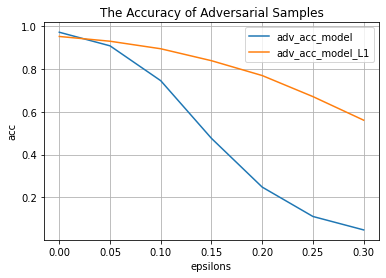
\includegraphics[width=6 cm]{softmax_modelL1.png}
\caption{Accuracy of the original model and the model 'Weight Decay'}
\label{softmax_L1}
\end{minipage}
\begin{minipage}[t]{0.48\textwidth}
\centering
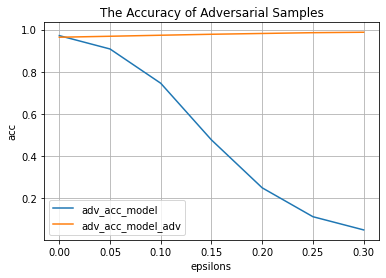
\includegraphics[width=6cm]{softmax_model_adv_ex.png}
\caption{Accuracy of the original model and the model 'adversarial examples'}
\label{softmax_adv}
\end{minipage}
\end{figure}
We can see that the adversarial training model is more robust to perturbations, but this adversarial training does not resist perturbations well (accuracy only 56\%) because the weights decay in the softmax regression case overestimating the damage that perturbations may achieve.

We then used another adversarial training method to train the model by creating a training set containing both adversarial and clean examples. And compare the accuracy of the original model and the adversarial training model (cf.FIGURE \ref{softmax_adv}) We can see that the model is robust to perturbations after training with adversarial examples, and even the stronger the perturbation, the higher the accuracy. The current ratio of adversarial examples to clean examples in the training set is 1:1, and we speculate that the ratio will affect the accuracy, which we will verify in the follow-up.\\

For the logistic regression network, since there is no suitable binary database, we decided to sample the Mnist database by extracting images with 0 and 1 information to form a new database. The above experimental steps were repeated. We observed that the linear regression network is far more resistant to interference than the other networks, and therefore in that experiment, an L1 penalty with a weight decay factor of -0.5 is added for adversarial training (the maximum value of the perturbation parameter epsilon is 0.5).(cf.FIGURE \ref{RL_L1})
\begin{figure}[htb]
\centering
\begin{minipage}[t]{0.48\textwidth}
\centering
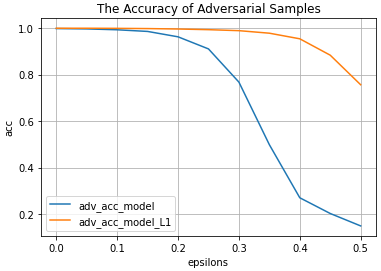
\includegraphics[width=6 cm]{Acc of RL l1.png}
\caption{Accuracy of the original model and the model 'Weight Decay'}
\label{RL_L1}
\end{minipage}
\begin{minipage}[t]{0.48\textwidth}
\centering
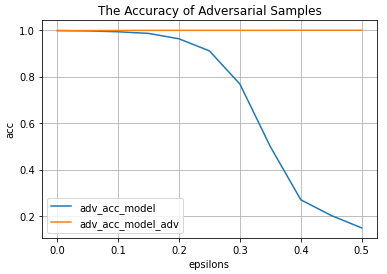
\includegraphics[width=6cm]{Acc of RL adv.png}
\caption{Accuracy of the original model and the model 'adversarial examples'}
\label{RL_adv}
\end{minipage}
\end{figure}
We were surprised to find that the adversarial training of the linear regression network was very effective, with an accuracy of 98\% at a perturbation of 0.3, compared to 80\% for the untrained network. At a perturbation of 0.5, the trained network achieves 63\% accuracy, while the accuracy of the untrained network is already reduced to 14\%. In addition, the linear regression network was much more resistant to perturbations than the other networks, still achieving 63\% accuracy at a perturbation of 0.3, while the accuracy of the other networks had dropped to 10\% at that point. (cf.FIGURE \ref{RL_L1})
\subsubsection{Discussion}
\FloatBarrier
\begin{figure}[htbp]
        \centering
        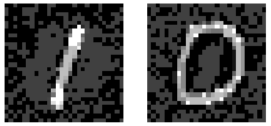
\includegraphics[width=5cm]{gradiant.PNG}%height=2cm,width=3cm,
        \caption{Image with the adversarial example}
        \label{gradient}
\end{figure}\par
\FloatBarrier
The principle of FGSM is  to increase the loss in the steepest direc of the gradient. This is a very abstract explanation, but perturbations for binary networks explain the concept very intuitively. As shown above, the physical shape of the perturbation in image 1 is the opposite of the perturbation in image 2 (cf.FIGURE \ref{gradient}), since a perturbation for either class in a binary network is meant to mislead the neural network into classifying it into another class, so the form of the perturbation is reasonable.


\subsection{Deep Neural Network}
\subsubsection{Description of the experience}
\href{https://github.com/LIUHanlin16895/MLA_projet/blob/main/src/maxout/ProjetMLAmaxoutFGSM.ipynb}{Lien github: Maxout} \\

%\textbf{Description de l'expérience réalisée, méthodologie et métriques d'évaluation.} \\
It is clear that standard supervised training does not specify that the chosen loss function be resistant to adversarial examples. This has to be encoded in some way during the training process. In this section, we used two kinds of adversarial training on a simple network (maxout) to improve its robustness. First we added the adversarial loss to the loss function. As described in the paper, its form is as follows :
$$ f_{adv}(\theta,x,y) = \alpha f(\theta,x,y) +(1-\alpha )f(\theta,x+\epsilon sign(\nabla_{x}f(\theta,x,y),y) $$
As in the paper, we take $\alpha$ always as 0.5. Its role is similar to an effective regularizer. This means that we will constantly update the adversarial sample in our training. We generate adversarial samples at the end of each batch and calculate the losses caused by them. After that we use the obtained new losses to compute the gradient and propagate.

In the second approach, first we trained a model without adversarial training. Then, we generated the corresponding adversarial samples and added these samples to the training set. We used this training set with the adversarial samples to re-train our model. This approach is similar to data augmentation. 


%\lipsum[4]

\subsubsection{Résultats}
%\textbf{Présentation des résultats expérimentaux obtenus et  comparaison par rapport à ceux de l’article de réference.} \\
In this section, we repeated the experiments in the paper and compare the results obtained with those in the original paper. In the first adversarial training we found a significant increase in training time because the number of samples in each batch is doubled in this approach. However, we did not achieve the same results on the test set. First, in the maxout network paper\citep{pmlr-v28-goodfellow13}, the authors achieved an accuracy of 99.06 $\%$ using the simple structure of MLP+maxout+dropout. However, in the github code given by the authors, dropout is not used and the final accuracy is only 97.3$\%$. The best accuracy we have found in other replications is 98.5$\%$. Our accuracy is 98.4$\%$ after fifty epochs, which is similar to Maxime Vandegar.

By using eraly stopping, we had an average error rates of 1.35 $\%$ with adversarial training and the best error rate of 1.26 $\%$, which are better than error rates without adversarial training (1.7$\%$). After confirming that the adversarial regular term improves the performance of the model on the original training set, we studied whether the model is robust to adversarial samples. The results are shown in Figure \ref{acc_advtraining_2}.

\begin{figure}[htbp]
\centering
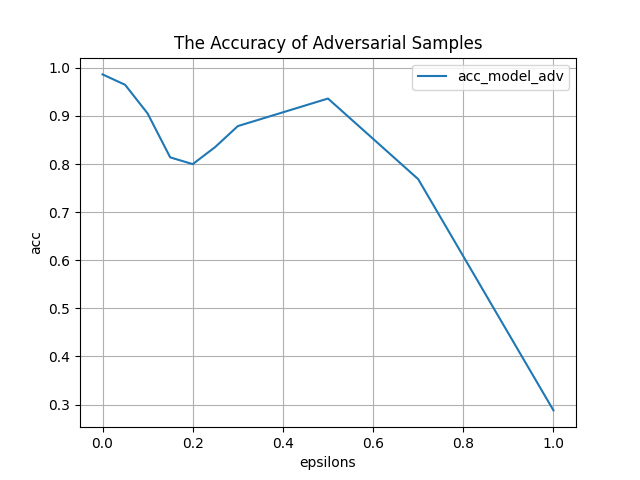
\includegraphics[width=6cm]{acc_advtraining_2.png}
\caption{Accuracy of model with adversarial training}
\label{acc_advtraining_2}
\end{figure} 
%\lipsum[5]

We reduced the error rate from 89.4$\%$ to 19.6$\%$, which is the highest error with $\epsilon = 0.2$ for all perturbations imperceptible to humans ($\epsilon < 0.5$).
\subsubsection{Discussion}
We observed that weights changed significantly, and the weights of the models with adversarial training were significantly more limited and interpretative. We can considered adversarial training as adding noise. And our model mined hardly in noisy inputs in order to train more efficiently by considering only those noisy points that strongly resist classification. This regularizer is efficient because the derivative of the sign function is zero or undefined. As loss function of our model is based on gradient descent, it could not react to changes in the parameter. We can also apply adversarial perturbations on hidden layer, it's less efficient. And apply adversarial perturbations on last layer didn't work. 
%\textbf{Discussion critique à partir des résultats obtenus} \\

%\subsection{Model Capacity}
%Model capacity refers to the ability of a machine learning model to capture and represent complex patterns in the data it is trained on. A model with high capacity is one that is able to learn and represent a wide range of patterns, while a model with low capacity is one that can only learn and represent a limited range of patterns. In the context of adversarial examples, models with high capacity are more susceptible to being fooled by adversarial inputs. Understanding and controlling the capacity of machine learning models can help improve the robustness and reliability of machine learning systems.

%\subsection{Adversarial Examples}
%Adversarial examples are inputs to machine learning models that have been specifically crafted to cause the model to make a mistake. These inputs are carefully constructed to be very similar to typical inputs, but with just a small, carefully chosen perturbation added. Because of this, adversarial examples can be challenging for machine learning models to handle. One of the key properties of adversarial examples is that they often generalize to other models and other tasks. This means that an adversarial example that is able to fool one model might also be able to fool other models that are trained on the same or similar data. There are several reasons why adversarial examples tend to generalize. Researchers and practitioners are working on developing techniques to better understand and control the generalization of adversarial examples.

%\subsection{Alternative Hypotheses}
%One hypothesis for explaining and harnessing adversarial examples is that generative training could provide more constraint on the training process, or cause the model to learn to distinguish "real" from "fake" data and be confident only on "real" data. Generative training refers to a type of training that is used to teach a machine learning model to generate new data that is similar to the data it has been trained on. The hypothesis is that by using generative training, it might be possible to constrain the model's learning process in a way that makes it less susceptible to adversarial examples. This is an active area of research.
%Another hypothesis for why adversarial examples exist is that individual models have strange quirks, but averaging over many models can cause adversarial examples to wash out. This hypothesis suggests that the reason adversarial examples are able to fool individual models is because each model has its own unique characteristics and quirks, which can make it more or less susceptible to adversarial inputs. However, when many models are combined, these quirks can cancel each other out, causing the ensemble of models to be more robust and less susceptible to adversarial examples. This hypothesis is supported by empirical evidence.
%\lipsum[6]


